\documentclass[Lau, oneside]{sapthesis}%remove "english" for a thesis written in Italian
\graphicspath{ {images/} }
%Bachelor's (laurea triennale) thesis : Lau 
%Master's (laurea specialistica) thesis: LaM 
%PhD's thesis: PhD 
\usepackage[italian]{babel} %use this package for a thesis written in Italian
\usepackage[utf8]{inputenx}
\usepackage{indentfirst}
\usepackage{microtype}
%\usepackage{chemformula}
%\usepackage{setspace}
%\usepackage{yfonts,color}https://www.overleaf.com/project/5e4187442ef81c00013a37ea
%\usepackage{siunitx}
%\usepackage{comment}
%\usepackage{multirow}
%\usepackage{varioref}
%\usepackage[bottom]{footmisc}
%\usepackage{wrapfig}
%\usepackage{float}
%\usepackage{type1cm}
\usepackage{lettrine}
%portare linespread a 1.1-1.3
\linespread{1.1}
%\usepackage{chngcntr}
\usepackage[nottoc, notlof, notlot]{tocbibind}
%\onehalfspacing
%\counterwithout{footnote}{chapter}
\usepackage{hyperref}
\hypersetup{
			hyperfootnotes=true,			
			bookmarks=true,			
			colorlinks=true,
			linkcolor=red,
                        linktoc=page,
			anchorcolor=black,
			citecolor=red,
			urlcolor=blue,
			pdftitle={Sviluppo App},
			pdfauthor={Edoardo Gabrielli},
			pdfkeywords={thesis, sapienza, roma, university}
 }

\title{Sviluppo App}
\author{Edoardo Gabrielli}
\IDnumber{1693726}
\course[]{Informatica}
\courseorganizer{Facolt\`a di Ingegneria dell’Informazione, Informatica e Statistica}
\submitdate{2019/2020}
\copyyear{2020}
\advisor{Prof. Emanuele Panizzi}
\authoremail{gabrielli.1693726@studenti.uniroma1.it}
\examdate{23 marzo 2020}
\examiner{Prof.}

%we refer to http://ctan.mirrorcatalogs.com/macros/latex/contrib/sapthesis/sapthesis-doc.pdf for an exhaustive description of the sapthesis documentclass.


\begin{document}

\frontmatter
\maketitle
\begin{abstract}
Oggetto della tesi è lo sviluppo delle app InfoStud e InfoProf in cui mi sono occupato di risolvere i problemi pre-esistenti e aggiungere nuove funzionalità di entità variabile.
Il documento è diviso in tre macro aree: un'introduzione generale alle applicazioni, al processo di sviluppo e agli strumenti utilizzati, poi l'iniziale attività di bug-fixing che comprende anche l'aggiunta di piccole features e infine una parte dedicata allo studio, progettazione ed implementazione dell'apertura di un verbale d'esame.
\end{abstract}

\tableofcontents

\mainmatter
\chapter{Introduzione}
\label{ch:1}

\section{InfoStud e InfoProf}
\label{sec:pres}
L'app InfoStud nasce \textit{n} anni fa dalla necessità degli studenti di avere il sistema InfoStud sviluppato da InfoSapienza su mobile.
Data la natura poco \textit{mobile-friendly} del sistema web, nacque l'app ufficiale sotto il brand di SapienzaApps.

SapienzaApps, sotto il coordinamento del Prof. Emanuele Panizzi, pubblica e mantiene progetti come SeismoCloud e GeneroCity all'interno
del Gamification Lab.

InfoStud è l'app che si rivolge unicamente agli studenti iscritti alla Sapienza e mette a disposizione un parco di funzionalità ampio
che copre le funzioni standard del sistema padre (come visualizzazione e gestione esami) e andando oltre in alcuni casi: il sistema
di gestione dell'orario didattico semi-automatico, la compilazione dei bollettini automatica, la prenotazione dei posti in biblioteca, ecc.

InfoProf, al contrario, è l'app che si rivolge ai professori della Sapienza e vuole essere uno strumento alternativo, e più intuitivo, 
del sistema web. La semplicità di utilizzo dell'app va però analizzata e progettata in modo empirico. Questo studio porta via molto tempo 
al lavoro ed è per questo che gran parte della progettazione si traduce in prototyping e test di usabilità, con eventualmente molteplici
iterazioni. Lo stato dell'arte attualmente è un'app che permette di verbalizzare gli studenti, attivare gli OPIS e cercare le aule.
Queste funzionalità hanno un denominatore in comune: sono casi d'uso in cui l'utente potrebbe non avere il computer quando ha bisogno
di utilizzarle. La verbalizzazione infatti può essere fatta subito dopo un orale, senza dover aspettare di tornare in ufficio e 
registrare i voti di tutti gli studenti. L'OPIS, date le ultime disposizioni, deve essere attivato durante la lezione, ma un utente
potrebbe non voler portare un computer in aula solo per attivare il codice OPIS.

Il mio tirocinio, in larga parte, è stato composto dall'aggiunta di piccole funzionalità richieste dall'utenza o dalla risoluzione di 
problemi: su InfoStud mi sono occupato di migliorare il login, aggiungere un'icona su SmartBiblio per indicare i posti non gestiti
dal sistema, migliorare la dark-mode e aggiungere l'immagine del profilo nel menù laterale. Su InfoProf invece ho lavorato alla
traduzione automatica, anche qui sul login, sul date-picker nella registrazione del voto di un esame e infine sul vero protagonista del 
tirocinio, ovvero l'apertura di un verbale, in cui ho fatto uno studio più approfondito di cui parlerò in \ref{ch:3}.

\section{Perché?}
\label{sec:why}
%trovare articoli scientifici in merito. 
Lo smartphone è ormai uno strumento radicato nella nostra quotidianeità. Sono innumerevoli i modi in cui ha cambiato la nostra vita e la
produttività è uno degli aspetti centrali. Nel settore pubblico l'evoluzione dei sistemi informatici però pecca di una rigorosa analisi 
e progettazione, il che comporta perdite di tempo e difficoltà nell'utilizzo.
Dall'indagine preliminare che ho svolto infatti emerge che alcuni intervistati trovano l'interfaccia web \textit{error-prone}, mentre 
un professore assunto recentemente, ha dichiarato che la piattaforma non è affatto user-friendly e che la logica vorrebbe che ci fosse
un tasto "crea appello", non che debba andarlo a cercare in "verbalizzazione". Anche all'interno del team di sviluppo, quando ci è
stata presentata per la prima volta l'interfaccia, abbiamo faticato a capire come svolgere i task che un professore è tenuto normalmente
a fare. Tolti errori grossolani come l'assegnazione di termini differenti alla stessa cosa [trovare un termine più adatto] 
\textbf{(inserire figura)}, esistono delle criticità che vanno contro la logica comune: se andiamo ad osservare la lista degli insegnamenti,
alla destra di ogni elemento possiamo osservare un numero che rappresenta il numero di \textit{corsi} selezionati accoppiati con quell'
insegnamento. Se selezioniamo il checkbox dell'elemento e andiamo all'interno del sotto-menù, deselezionando tutti i corsi, l'insegnamento
rimarrà selezionato. Una buona interfaccia \textbf{(citare)}, invece, dovrebbe aiutare l'utente ad evitare gli errori.

%citare le statistice del miur riguardo età e numero di docenti della sapienza

%L'approccio che ho avuto quindi è stato quello di capire cosa gli utenti ritengono più importante nell'apertura di un verbale e mettere
%in secondo piano le funzionalità che vengono usate raramente. Vedremo infatti che paradossalmente l'interfaccia web, ai docenti che 
%hanno imparato ad usarla, piace.


\chapter{Metodologie di sviluppo}
\label{ch:2}

\section{Organizzazione}
\label{sec:team}
Il team è composto da studenti impiegati nello sviluppo per circa tre mesi. E' prassi iniziare ad ambientarsi nei progetti attraverso
l'attività di bug-fixing: familiarizzare con il codice e con i colleghi è centrale dato che per molti di noi è la prima esperienza
dentro un progetto di discrete dimensioni e all'interno di un contesto semi-professionale.

La metodologia di sviluppo che si adatta meglio alle nostre esigenze è l'Agile, il quale si basa su un insieme di regole il cui senso
generale è un approccio adatto ai cambiamenti, non fisso e rigoroso, che misura i progressi attraverso codice funzionante e incoraggia 
il rilascio continuo del software per soddisfare l'utente finale. 

Un aspetto fondamentale che si ricollega a questo è l'integrazione
continua del codice prodotto dagli sviluppatori: nel laboratorio utilizziamo GitLab, un sistema di controllo versione che tiene
traccia delle modifiche, segnala i conflitti che possono generarsi dalla modifica simultanea dello stesso file e aiuta a gestire i compiti 
del singolo sviluppatore.
Ad ogni \textit{merge request}, le modifiche apportate al codice sono revisionate da un controllo umano che garantisce la qualità del codice.
Se infatti lo stile non è coerente con il resto del progetto, se ci sono bug introdotti dalle modifiche o altri problemi, la merge request 
viene respinta.

\section{Tecnologie utilizzate}
\label{sec:tech}
Per sviluppare il front-end delle app utilizziamo Ionic Framework v3, che è basato su AngularJS. Ionic permette di utilizzare tecnologie
web per creare interfacce secondo gli standard di Android e iOS. Il vantaggio dell'uso di Angular è che il codice non va adattato ad alcuna
piattaforma, inoltre per chiunque abbia già una discreta conoscenza della programmazione web è immediato iniziare a programmare. Tutto
ciò velocizza molto la scrittura di una UI, ma bisogna fare dei compromessi: l'interfaccia non segue diligentemente gli standard imposti
dal Material Design o dall'iOS UI Design perchè deve adattarsi ad entrambe le piattaforme. Un'altra criticità è che di fatto l'app è
un'interfaccia web con caratteristiche \textit{app-like}, ovvero una Progressive Web App sviluppata in Angular. 
Il ruolo di Ionic è fornire gli elementi dei vari standard di design già fatti e di integrare anche le funzionalità native attraverso
Ionic Native o Cordova. Ciò significa che le prestazioni ne risentono ripetto ad un'app nativa. Inoltre ad oggi Ionic è alla versione 5,
ma è impossibile aggiornare i progetti senza andare a creare dei conflitti che vanno risolti manualmente, vista la mole di codice che è
stato scritto quindi, siamo costretti a rimanere ad una versione di qualche anno fa, all'occorenza programmando manualmente le novità
introdotte dagli standard.

InfoStud ed InfoProf sono progettati seguendo il pattern Model-View-Controller (MVC). Come dice il nome stesso, il pattern impone una 
separazione del software attraverso tre componenti:
\begin{itemize}
	\item Model: rappresentano le classi, contiengono i dati dell'applicazione a cui si accede attraverso i metodi che forniscono;
	\item View: la view accede ai dati forniti dai modelli e li presenta all'utente, inoltre comunica con i controller;
	\item Controller: il controller intercetta le azioni dell'utente attraverso la view ed è in grado di modificare i model. 
\end{itemize}

\begin{figure}[h]
	\caption{Schema del funzionamento del pattern MVC \cite{ref:mvc}.}
	\centering
	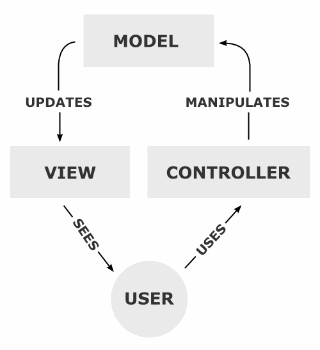
\includegraphics[width=0.5\textwidth]{MVC-Process}
	\label{fig:mvc}
\end{figure}

Ciò che traspare dunque è che la logica di business viene separata dalla logica di presentazione. Inoltre il pattern MVC incoraggia il 
lavoro di gruppo permettendo agli sviluppatori di lavorare simultaneamente su diversi aspetti dell'applicazione. Un'altro aspetto importante
riguardo il riuso del codice, infatti diverse view accedono agli stessi controller e modelli. Ad esempio, quando ho sviluppato l'immagine
del profilo nel menù laterale, mi è bastato accedere ad un metodo del provider %in realtà non è proprio mvc


\chapter{Progettazione}
\label{ch:3}
%inserire diagramma di flusso di come viene fatta la progettazione (nf -> protoryping -> test -> repeat)

\section{Need-finding}
\label{sec:nf}

\section{Progettazione della UI}
\label{sec:ui}
%citare "Developing SMASH"

\section{Implementazione}
\label{sec:dev}
%inserire qualche snippet e magari parlare dei limiti tecnologici di ionic e come li ho superati


\chapter{Concluzioni}
\label{ch:4}

\backmatter
\phantomsection
\begin{thebibliography}{17}

\bibitem{ref:mvc}
Tratto da Wikipedia:
https://it.wikipedia.org/wiki/Model-view-controller

\end{thebibliography}

\end{document}